% --- INSTITUTIONAL TEMPLATE FED v7.4.9 ---
% Estándar de Reporteo APA 7 (Babel-Free)
\documentclass[12pt,spanish]{article}

\usepackage{graphicx}
\usepackage{geometry}
\usepackage{indentfirst} 
\usepackage{caption}
\usepackage{floatrow} 

% Forzar estilos de caption antes de cualquier carga
\floatsetup[figure]{capposition=top}
\floatsetup[table]{capposition=top}

\usepackage{booktabs}
\usepackage{float}
\usepackage{longtable}
\usepackage{threeparttable}
\usepackage{array}
\usepackage{calc}
\usepackage{amsmath, amssymb}
\usepackage{fancyhdr}
\usepackage{mathptmx} 
\usepackage[T1]{fontenc}
\usepackage{setspace} 
\usepackage{ragged2e} 
\usepackage{titlesec}
\usepackage{url}
\def\UrlBreaks{\do\/\do-\do\.\do\_\do\?\do\=\do\&\do\%}
\usepackage[hidelinks,breaklinks]{hyperref}
\usepackage{xcolor}
\usepackage{fancyvrb}
\usepackage{framed}

% --- Code Highlighting (Pandoc Standard) ---
\newenvironment{Shaded}{\begin{snugshade}}{\end{snugshade}}
\definecolor{shadecolor}{RGB}{248,248,248}
\newenvironment{Highlighting}{}{}
\newcommand{\VerbBar}{|}
\newcommand{\VERB}{\Verb[commandchars=\\\{\}]}
\DefineVerbatimEnvironment{Highlighting}{Verbatim}{commandchars=\\\{\}}
\newcommand{\AlertTok}[1]{\textcolor[rgb]{0.94,0.16,0.16}{#1}}
\newcommand{\AnnotationTok}[1]{\textcolor[rgb]{0.56,0.35,0.01}{\textbf{\textit{#1}}}}
\newcommand{\AttributeTok}[1]{\textcolor[rgb]{0.13,0.29,0.53}{#1}}
\newcommand{\BaseNTok}[1]{\textcolor[rgb]{0.00,0.00,0.81}{#1}}
\newcommand{\BuiltInTok}[1]{#1}
\newcommand{\CharTok}[1]{\textcolor[rgb]{0.31,0.60,0.02}{#1}}
\newcommand{\CommentTok}[1]{\textcolor[rgb]{0.56,0.35,0.01}{\textit{#1}}}
\newcommand{\CommentVarTok}[1]{\textcolor[rgb]{0.56,0.35,0.01}{\textbf{\textit{#1}}}}
\newcommand{\ConstantTok}[1]{\textcolor[rgb]{0.56,0.35,0.01}{#1}}
\newcommand{\ControlFlowTok}[1]{\textcolor[rgb]{0.13,0.29,0.53}{\textbf{#1}}}
\newcommand{\DataTypeTok}[1]{\textcolor[rgb]{0.13,0.29,0.53}{#1}}
\newcommand{\DecValTok}[1]{\textcolor[rgb]{0.00,0.00,0.81}{#1}}
\newcommand{\DocumentationTok}[1]{\textcolor[rgb]{0.56,0.35,0.01}{\textbf{\textit{#1}}}}
\newcommand{\ErrorTok}[1]{\textcolor[rgb]{0.64,0.00,0.00}{\textbf{#1}}}
\newcommand{\ExtensionTok}[1]{#1}
\newcommand{\FloatTok}[1]{\textcolor[rgb]{0.00,0.00,0.81}{#1}}
\newcommand{\FunctionTok}[1]{\textcolor[rgb]{0.13,0.29,0.53}{\textbf{#1}}}
\newcommand{\ImportTok}[1]{#1}
\newcommand{\InformationTok}[1]{\textcolor[rgb]{0.56,0.35,0.01}{\textbf{\textit{#1}}}}
\newcommand{\KeywordTok}[1]{\textcolor[rgb]{0.13,0.29,0.53}{\textbf{#1}}}
\newcommand{\NormalTok}[1]{#1}
\newcommand{\OperatorTok}[1]{\textcolor[rgb]{0.81,0.36,0.00}{\textbf{#1}}}
\newcommand{\OtherTok}[1]{\textcolor[rgb]{0.56,0.35,0.01}{#1}}
\newcommand{\PreprocessorTok}[1]{\textcolor[rgb]{0.56,0.35,0.01}{\textit{#1}}}
\newcommand{\RegionMarkerTok}[1]{#1}
\newcommand{\SpecialCharTok}[1]{\textcolor[rgb]{0.81,0.36,0.00}{\textbf{#1}}}
\newcommand{\SpecialStringTok}[1]{\textcolor[rgb]{0.31,0.60,0.02}{#1}}
\newcommand{\StringTok}[1]{\textcolor[rgb]{0.31,0.60,0.02}{#1}}
\newcommand{\VariableTok}[1]{\textcolor[rgb]{0.00,0.00,0.00}{#1}}
\newcommand{\VerbatimStringTok}[1]{\textcolor[rgb]{0.31,0.60,0.02}{#1}}
\newcommand{\WarningTok}[1]{\textcolor[rgb]{0.56,0.35,0.01}{\textbf{\textit{#1}}}}

% --- Pandoc Compatibility Block (Iron Clad) ---
\providecommand{\tightlist}{%
  \setlength{\itemsep}{0pt}\setlength{\parskip}{0pt}}

% Compatibilidad Pandoc 3.x
\ifdefined\pandocbounded\else
  \newcommand{\pandocbounded}[1]{#1}
\fi

% --- Pandoc Citeproc (CSL) compatibility ---
\newlength{\cslhangindent}
\setlength{\cslhangindent}{1.27cm} 
\newlength{\csllabelwidth}
\setlength{\csllabelwidth}{3em}
\newcommand{\citeproctext}{} 
\newcommand{\citeprocitem}[2]{\item} 
\newenvironment{CSLReferences}[2] 
 {\begin{list}{}{
  \setlength{\leftmargin}{\cslhangindent}
  \setlength{\parsep}{0pt}
  \setlength{\itemsep}{6pt}
  \ifodd #1
   \setlength{\leftmargin}{\leftmargin + \csllabelwidth}
   \setlength{\itemindent}{-\csllabelwidth}
  \fi
  }
  \renewcommand{\bibitem}[2][]{\item} % Elimina los corchetes [ ]
 }
 {\end{list}}
\newcommand{\CSLBlock}[1]{#1\hfill\break}
\newcommand{\CSLLeftMargin}[1]{\parbox[t]{\csllabelwidth}{#1}}
\newcommand{\CSLRightInline}[1]{\parbox[t]{\linewidth - \csllabelwidth}{#1}\break}
\newcommand{\CSLIndent}[1]{\hspace{\cslhangindent}#1}

\makeatletter
\@ifundefined{paragraph}{\newcounter{paragraph}}{}
\@ifundefined{subparagraph}{\newcounter{subparagraph}}{}
\makeatother

% Solución al error 'No counter none defined' en longtable
\makeatletter
\newcounter{none}
\@ifpackageloaded{caption}{
  \DeclareCaptionType{none}
  \captionsetup[none]{name=Tabla}
}{}
\makeatother

\hypersetup{
  colorlinks=true,
  linkcolor=blue,
  filecolor=blue,
  citecolor=blue,
  urlcolor=blue
}

% --- Macros Institucionales ---
\newcommand{\fuente}[1]{
  \vspace{4pt}
  \begin{flushleft}
    \small
    \textit{Nota.} #1
  \end{flushleft}
}

% --- Localización Manual Determinista (Sin Babel) ---
\AtBeginDocument{
  \renewcommand{\tablename}{Tabla}
  \renewcommand{\figurename}{Figura}
  \renewcommand{\contentsname}{Índice}
  \renewcommand{\listtablename}{Índice de Tablas}
  \renewcommand{\listfigurename}{Índice de Figuras}
  \renewcommand{\abstractname}{Resumen}
  \renewcommand{\refname}{Referencias}
  
  \RaggedRight
  \setlength{\parindent}{1.27cm}
  \setlength{\parskip}{0pt}
}

\DeclareCaptionLabelSeparator{newline}{\\ \vspace{2pt}}
\captionsetup{
  position=top,
  justification=RaggedRight,
  singlelinecheck=false,
  labelfont=bf,
  textfont=it,
  labelsep=newline,
  font=small,
  skip=10pt
}
\captionsetup[figure]{name=Figura}
\captionsetup[table]{name=Tabla}

% Márgenes APA 7
\geometry{
  a4paper,
  margin=25.4mm,
  headheight=15mm
}

% --- Encabezados ---
\pagestyle{fancy}
\fancyhf{} 
\fancyhead[L]{
\includegraphics[height=1.2cm]{/home/erick-fcs/Capital_Workstation/capital-workstation-libs/src/ecs_quantitative/reporting/assets/logos/logo_unl.png}}
\fancyhead[R]{
\includegraphics[height=1.2cm]{/home/erick-fcs/Capital_Workstation/capital-workstation-libs/src/ecs_quantitative/reporting/assets/logos/logo_economia.jpg}}
\renewcommand{\headrulewidth}{0pt}
\fancyfoot[R]{\thepage}

\fancypagestyle{plain}{
  \fancyhf{}
  \fancyhead[L]{
\includegraphics[height=1.2cm]{/home/erick-fcs/Capital_Workstation/capital-workstation-libs/src/ecs_quantitative/reporting/assets/logos/logo_unl.png}}
  \fancyhead[R]{
\includegraphics[height=1.2cm]{/home/erick-fcs/Capital_Workstation/capital-workstation-libs/src/ecs_quantitative/reporting/assets/logos/logo_economia.jpg}}
  \fancyfoot[R]{\thepage}
  \renewcommand{\headrulewidth}{0pt}
}

% --- Títulos ---
\titleformat{\section}{\normalfont\normalsize\bfseries\centering}{\thesection}{1em}{}
\titleformat{\subsection}{\normalfont\normalsize\bfseries}{\thesubsection}{1em}{}
\titleformat{\subsubsection}{\normalfont\normalsize\bfseries\itshape}{\thesubsubsection}{1em}{}
\titlespacing*{\section}{0pt}{12pt}{6pt}
\titlespacing*{\subsection}{0pt}{12pt}{6pt}
\titlespacing*{\subsubsection}{0pt}{12pt}{6pt}

\newenvironment{referenciasAPA}{
  \setlength{\parindent}{-1.27cm}
  \setlength{\leftskip}{1.27cm}
  \setlength{\parskip}{6pt}
}{\par}

\begin{document}

\begin{center}
    {\bfseries \Large Universidad Nacional de Loja}\\[0.3cm]
    {\bfseries \large Facultad Jurídica, Social y
Administrativa}\\[0.2cm]
    {\bfseries Carrera de Economía}\\[1.5cm]
    
    {\bfseries \large Econometría Aplicada}\\[1cm]
    
    {\bfseries \Large Evaluación de Impacto: Factores Determinantes de
la Violencia Letal en Ecuador (1990-2023)}\\[1.5cm]
\end{center}

\noindent {\bfseries Estudiante:} Erick Fabricio Condoy Seraquive \\
\noindent {\bfseries Docente:} Eco. José Rafael Alvarado López \\
\noindent {\bfseries Fecha:} 20 de abril de 2026 \\

\vspace{1cm}

\doublespacing
\setlength{\parindent}{1.27cm}

\section{Problema de Investigación}\label{problema-de-investigaciuxf3n}

Ecuador ha experimentado una transformación violenta y acelerada en su
panorama de seguridad pública. Tras una década de reducción sostenida en
las tasas de homicidios (2011-2018), el país ingresó en una fase de
crisis caracterizada por un crecimiento exponencial de la violencia
letal, vinculada al crimen organizado transnacional. El problema radica
en que las políticas previas, como la prohibición de armas de 2011,
parecen haber perdido efectividad frente a las nuevas dinámicas
delictivas, generando la necesidad de un re-modelado econométrico que
capture estos quiebres estructurales.

\section{Teoría}\label{teoruxeda}

La investigación se sustenta en dos pilares teóricos: 1. \textbf{Teoría
de la Disuasión (Deterrence Theory):} Propone que el incremento del
``costo'' de cometer un crimen (como la restricción de medios para la
violencia, ej. armas) reduce la incidencia delictiva (Becker 1968). 2.
\textbf{Econometría del Crimen y Ruptura Institucional:} Analiza cómo
cambios en el entorno (pobreza, desempleo, fortaleza institucional)
alteran el equilibrio de violencia. En series temporales, esto se
manifiesta como quiebres estructurales donde las tendencias históricas
son invalidadas por nuevos choques externos (Shmueli 2010).

\section{Hipótesis}\label{hipuxf3tesis}

\begin{itemize}
\tightlist
\item
  \textbf{H1 (Hipótesis de Disuasión):} El Decreto 164 de 2011 generó un
  quiebre estructural negativo (reducción) en la tasa de homicidios
  inmediatamente después de su implementación.
\item
  \textbf{H2 (Hipótesis de Invalidez de Régimen):} Existe un segundo
  quiebre estructural a partir de 2019 que revirtió los logros de la
  política de 2011, causado por un cambio en la naturaleza delictiva del
  país.
\end{itemize}

\section{Descripción de Variables}\label{descripciuxf3n-de-variables}

Los datos provienen de la síntesis de microdatos de la ENEMDU (INEC) y
bases del Banco Mundial, centralizados bajo la arquitectura de la
librería \texttt{ecs\_quantitative}.

\begin{longtable}[]{@{}
  >{\raggedright\arraybackslash}p{(\linewidth - 6\tabcolsep) * \real{0.2500}}
  >{\raggedright\arraybackslash}p{(\linewidth - 6\tabcolsep) * \real{0.2500}}
  >{\raggedright\arraybackslash}p{(\linewidth - 6\tabcolsep) * \real{0.2500}}
  >{\raggedright\arraybackslash}p{(\linewidth - 6\tabcolsep) * \real{0.2500}}@{}}
\caption{Variables integradas para el diagnóstico de impacto en
seguridad}\label{tbl-vars-homicidios}\tabularnewline
\toprule\noalign{}
\begin{minipage}[b]{\linewidth}\raggedright
Variable
\end{minipage} & \begin{minipage}[b]{\linewidth}\raggedright
Tipo
\end{minipage} & \begin{minipage}[b]{\linewidth}\raggedright
Descripción
\end{minipage} & \begin{minipage}[b]{\linewidth}\raggedright
Fuente
\end{minipage} \\
\midrule\noalign{}
\endfirsthead
\toprule\noalign{}
\begin{minipage}[b]{\linewidth}\raggedright
Variable
\end{minipage} & \begin{minipage}[b]{\linewidth}\raggedright
Tipo
\end{minipage} & \begin{minipage}[b]{\linewidth}\raggedright
Descripción
\end{minipage} & \begin{minipage}[b]{\linewidth}\raggedright
Fuente
\end{minipage} \\
\midrule\noalign{}
\endhead
\bottomrule\noalign{}
\endlastfoot
\texttt{year} & Temporal & Año calendario de la observación (1990-2023)
& INEC \\
\texttt{homicidios\_100k} & Continuo & Tasa de muertes violentas por
cada 100k habitantes & INEC \\
\texttt{desempleo\_total\_ne} & Continuo & Tasa de desempleo nacional
(\%) & Banco Mundial \\
\texttt{gasto\_militar\_pct\_pib} & Continuo & Inversión en seguridad y
defensa respecto al PIB & Banco Mundial \\
\texttt{remesas\_pct\_pib} & Continuo & Flujo de remesas como proxy de
bienestar económico & Banco Mundial \\
\end{longtable}

\section{Metodología}\label{metodologuxeda}

Se implementa un modelo de \textbf{Series de Tiempo Interrumpidas (ITS)
de Doble Quiebre}. A diferencia del modelo estándar, esta especificación
captura dos regímenes distintos: la estabilización post-2011 y la
disrupción post-2019. Para corregir la autocorrelación detectada
(\(DW \approx 0.6\) en OLS simple), se emplean \textbf{Errores Estándar
Robustos HAC (Newey-West)}.

\[Y_t = \beta_0 + \beta_1 T_t + \beta_2 P_{1,t} + \beta_3 Q_{1,t} + \beta_4 P_{2,t} + \beta_5 Q_{2,t} + \epsilon_t\]

\section{Resultados}\label{resultados}

El refinamiento del modelo permitió elevar el coeficiente de
determinación \textbf{\(R^2\) de 0.33 a 0.91}, indicando que el doble
quiebre captura la verdadera estructura de la serie histórica.

\subsection{Impacto Inmediato (2011)}\label{impacto-inmediato-2011}

El efecto (\(\beta_2\)) tras la prohibición de 2011 fue una reducción
significativa de \textbf{-5.13 puntos} en la tasa de homicidios
(\(p < 0.001\)).

\subsection{Crisis de Seguridad
(Post-2019)}\label{crisis-de-seguridad-post-2019}

El cambio en la pendiente (\(\beta_5\)) post-2019 es de \textbf{+11.11},
indicando un crecimiento acelerado que invalida las tendencias previas.

\subsection{Análisis Gráfico}\label{anuxe1lisis-gruxe1fico}

\begin{figure}

\centering{

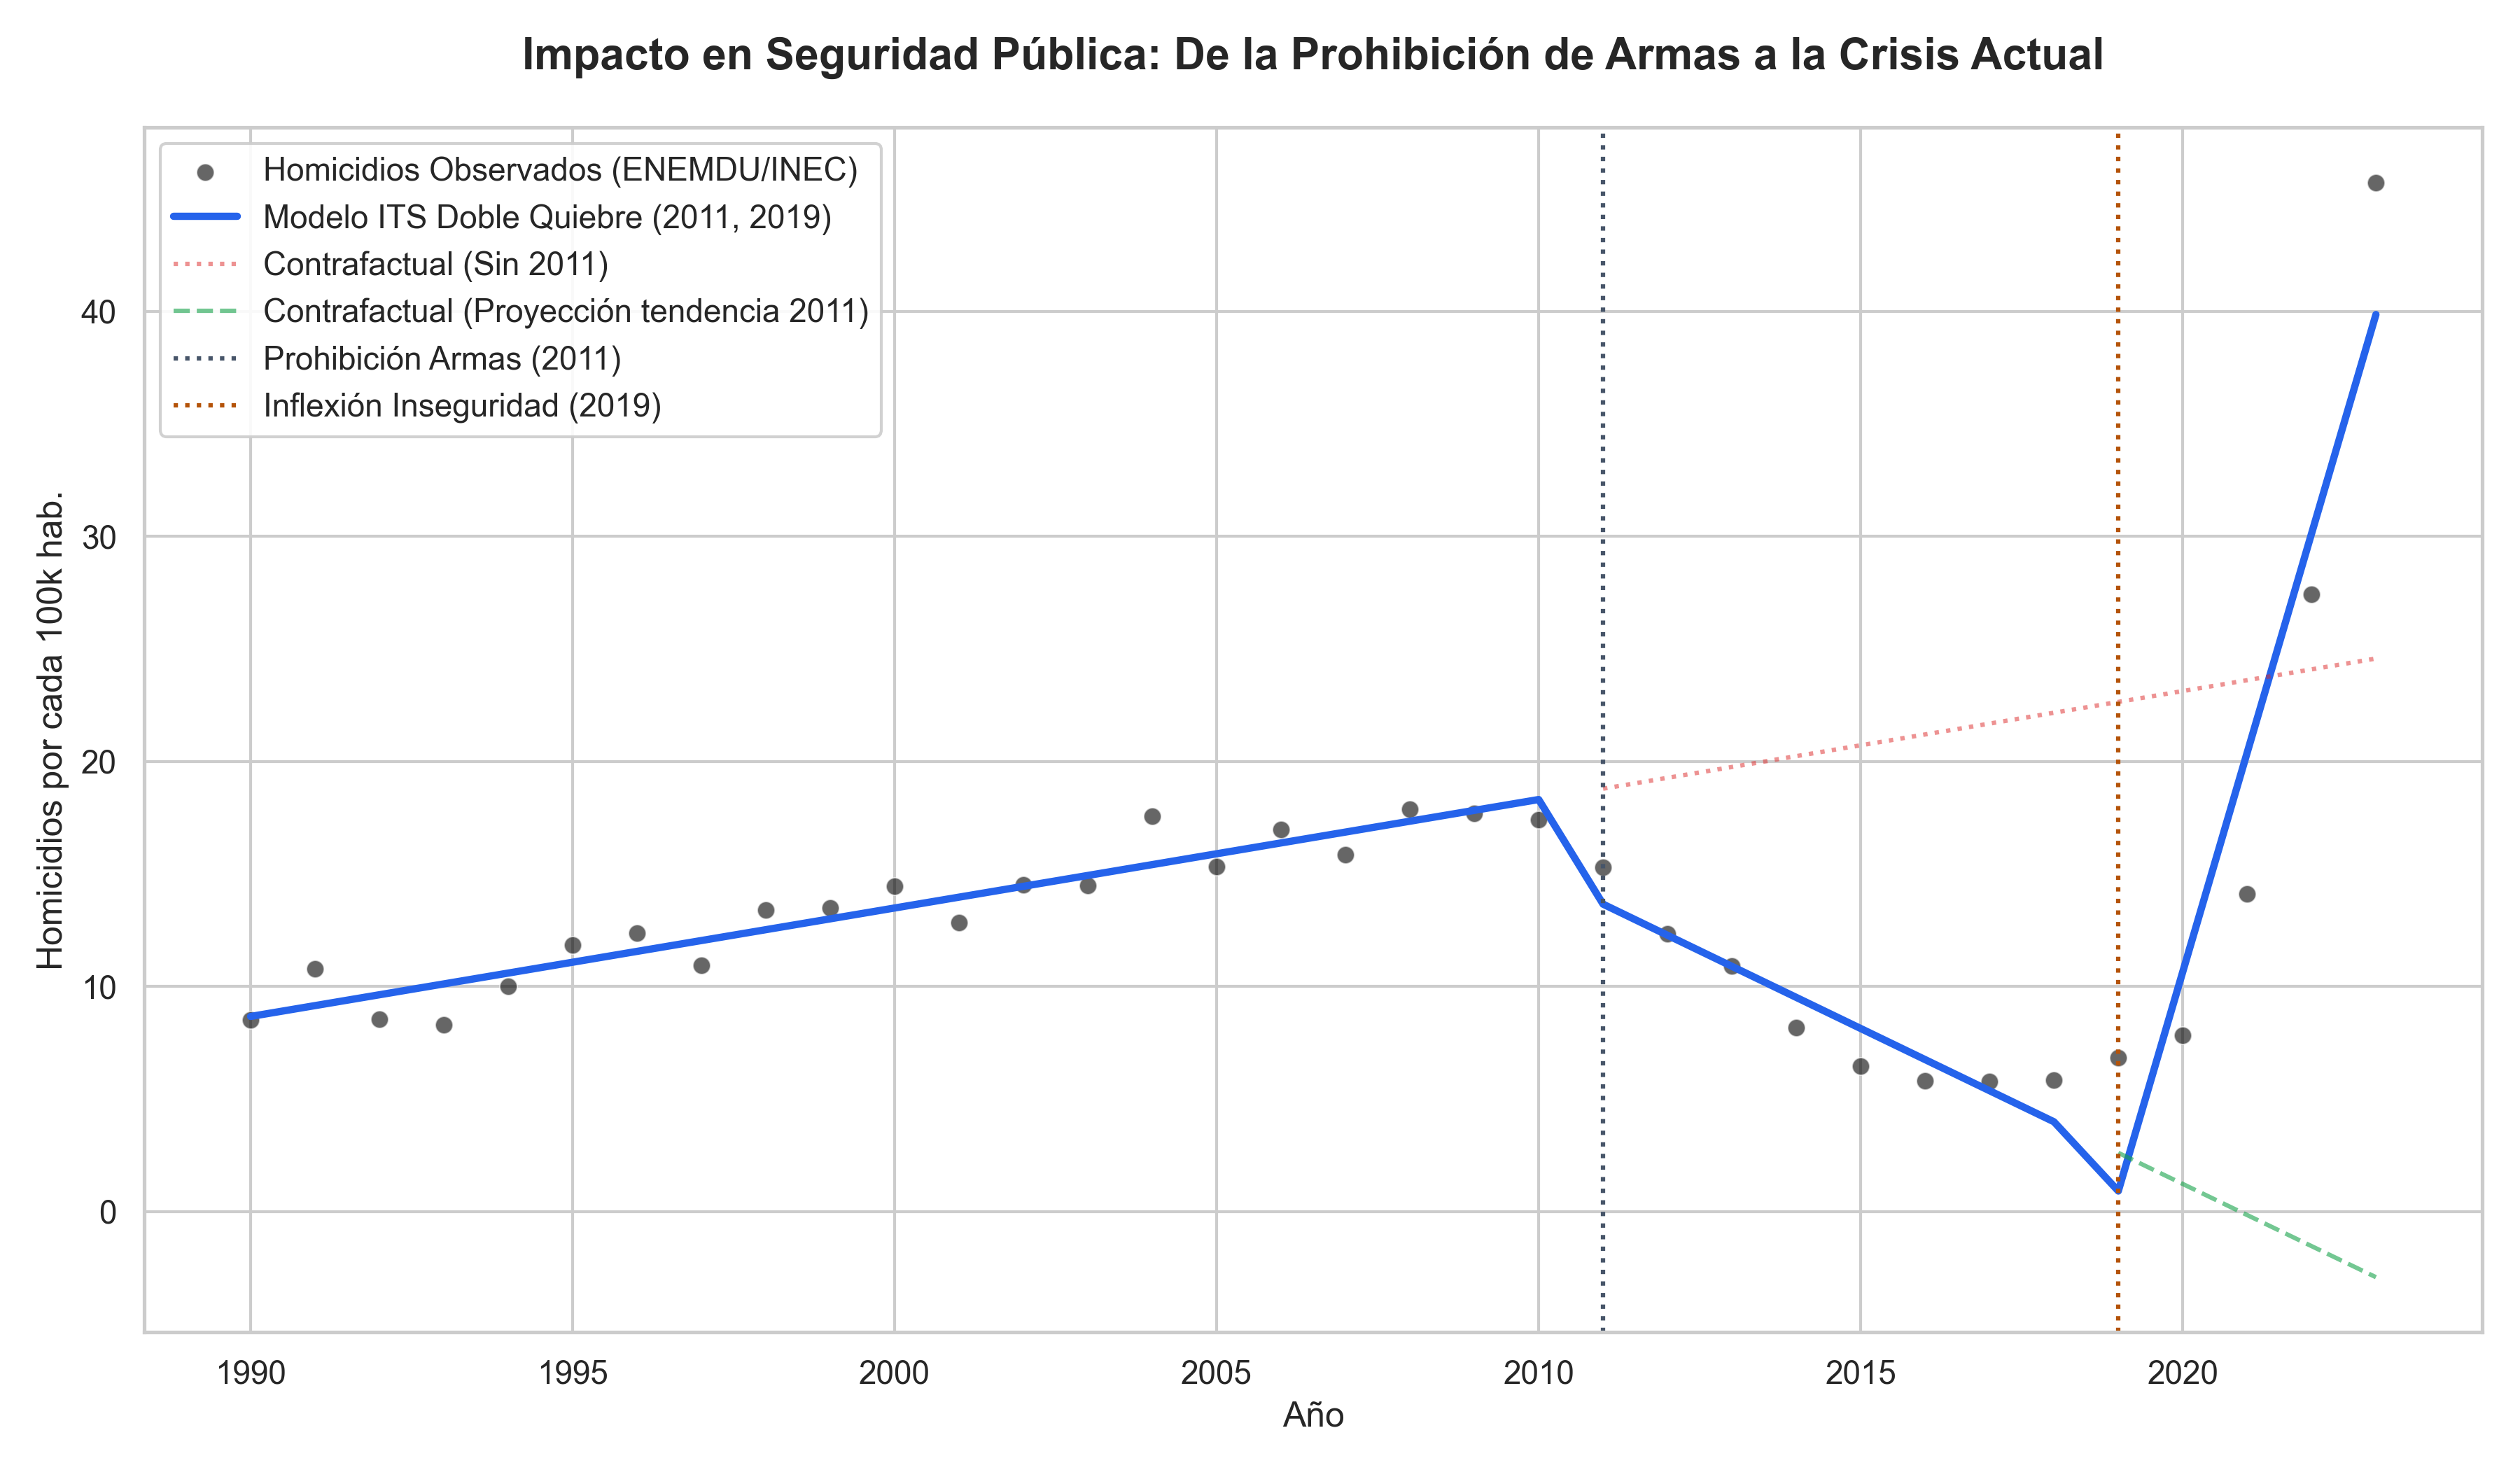
\includegraphics[width=0.75\linewidth,height=\textheight,keepaspectratio]{graph/impact_homicidios_its.png}

}

\caption{\label{fig-impacto}Homicidios en Ecuador: Modelo ITS Robusto
con Doble Inflexión}

\end{figure}%

\section{Conclusión}\label{conclusiuxf3n}

La prohibición de armas de 2011 fue eficaz en su contexto original. Sin
embargo, la actual crisis (post-2019) responde a una ruptura
institucional que trasciende el control de armas, exigiendo políticas de
seguridad de nueva generación.

\section{Referencias}\label{referencias}

\protect\phantomsection\label{refs}
\begin{CSLReferences}{1}{1}
\bibitem[\citeproctext]{ref-becker1968}
Becker, Gary S. 1968. {``Crime and Punishment: An Economic Approach.''}
\emph{Journal of Political Economy} 76 (2): 169--217.

\bibitem[\citeproctext]{ref-shmueli2010}
Shmueli, Galit. 2010. {``To Explain or to Predict?''} \emph{Statistical
Science} 25 (3): 289--310.

\end{CSLReferences}

\end{document}
